\documentclass[12pt, a4paper]{amsart} 
\usepackage[utf8]{inputenc}
\usepackage[spanish]{babel}
\usepackage{anysize}
\usepackage{amsthm}
\usepackage{multicol}
\newcommand{\noun}[1]{\textsc{#1}}
\usepackage{amsmath}
\usepackage{amsfonts}
\usepackage{amssymb}
\usepackage{graphicx}
\usepackage{amscd}
\usepackage[colorlinks=true,linktocpage=true,pagebackref=true, citecolor=red,linkcolor=blue]{hyperref}

%opening

\newtheorem{teorema}{Teorema}[section]
\newtheorem{definicion}[teorema]{Definición}
\newtheorem{prop}[teorema]{Proposición}
\newtheorem{obs}[teorema]{Observación}
\newtheorem{cor}[teorema]{Corolario}
\newtheorem{ejem}[teorema]{Ejemplo}
\newtheorem{ejems}[teorema]{Ejemplos}
\newtheorem{ejer}{Ejercicio}

\marginsize{2cm}{2cm}{1cm}{1cm}

\begin{document}
\thispagestyle{plain}

\title{Análisis. Ejercicios PAU CCSS II}

\date{}

\maketitle

\begin{ejer}\em (2021-2022)\\
a) Halle
\[\int_0^1 \frac{x}{2x^2+5}dx.\]
b) Considere
\[f(x)=\frac{x}{2x^2+5} \text{ y } g(x) = ln(x).\]
Halle la derivadade la función compuesta $f\circ g(x).$
\end{ejer}

\begin{ejer}\em (2021-2022)\\
Se considera la función $f(x)=\left \{ \begin{matrix}
ax^2 -1  & \text{si} & x \leq 1\\
(x-a)^2 & \text{si} & x> 1
\end{matrix}\right.
$
a) Determine los valores de $a\in\mathbb{R}$ que hacen que $f$ sea una función continua en su dominio.\\
b) Para $a = 1/2,$ determine, si existen, los puntos de corte de la gráfica de $f$ con el eje de las $x.$
\end{ejer}

\begin{ejer}\em (2021-2022)\\
Un ensayo clínico indica que la cantidad de glucosa en sangre en ratones tras la ingesta de un determinado fármaco depende del tiempo transcurrido, $t$ (en minutos), según la siguiente función
expresada en $mg/dl:$
\[f(t) = 90 + Ct^2e^{-t/5}, 0 \leq t \leq 60.\]
a) Obtenga razonadamente el valor de la constante $C$ sabiendo que la tasa de variación instantánea de la cantidad de glucosa a los 5 minutos de la ingesta del producto es $15/e.$\\
b) Para $C = 3,$ indique a partir de qué momento disminuye la cantidad de glucosa en sangre. Señale también la cantidad máxima de glucosa en sangre alcanzada tras la ingesta del fármaco.\\
Nota: Exprese los resultados con 2 cifras decimales.
\end{ejer}

\begin{ejer}\em (2021-2022)\\
Considere las funciones reales de variable real $f(x) = x^2 - 4x + 3$ y $g(x) = -x^2 + ax + 3.$\\
a) Se define $h(x)$ de la siguiente manera:
\[h(x)=\left \{ \begin{matrix}
f(x)  & \text{si} & x \leq 1\\
g(x) & \text{si} & x> 1
\end{matrix}\right.\]
¿Qué valor debe darle a la constante $a\in\mathbb{R}$ para que la función $h$ sea continua en $\mathbb{R}$?\\
b) Para $a = 2,$ halle el área de la región acotada del plano que está delimitada por las gráficas de $f$ y de $g.$
\end{ejer}

\begin{ejer}\em (2021-2022)\\
a) Determine los valores de los parámetros $a, b,\in \mathbb{R}$ para que la función $f(x)=ax+\frac{b}{x}$ verifique que $f(2) = 4$ y $f'(2)=0.$\\
b) Encuentre todas las asíntotas de la función $g(x) = x + \frac{1}{x}.$
\end{ejer}

\begin{ejer}\em (2021-2022)\\
Un investigador ha desarrollado un fertilizante para un determinado cultivo. Los estudios de mercado indican que los ingresos, $I(x),$ en miles de euros, vienen expresados por la función
\[I(x) = x\frac{170-0,85x}{5}\]
en la que x representa la demanda del producto, expresada en miles de litros. Por otra parte, los costes de producción que asume la empresa, en miles de euros, se expresan en función de la demanda mediante la función $C(x) = 10 + 2x + x^2.$\\
a) Proporcione una expresión para la función beneficio en términos de la demanda $x$ y encuentre la cantidad de producto que debería venderse para maximizarlo. Obtenga también el beneficio máximo.\\
b) Determine entre qué valores debería encontrarse la cantidad demandada de fertilizante para que el coste medio, $C(x)/x ,$ no supere los diez mil euros.\\
Nota: Exprese los resultados con 2 cifras decimales.
\end{ejer}

\begin{ejer}\em (2021-2022)\\
Se considera la función real de variable real 
\[
f(x)=\left \{ \begin{matrix}
2x-a  & \text{si} & x< -2\\
x^2 & \text{si} & -2\leq x \leq 1\\
x+b & \text{si} & 1< x
\end{matrix}\right.
\]
a) Determine los valores de $a$ y $b$ que hacen que $f$ sea continua en $\mathbb{R}.$\\
b) Para $a = b = -8,$ calcule
\[\int_{-3}^0f(x)dx.\]
\end{ejer}

\begin{ejer}\em (2021-2022)\\
La siguiente figura representa la gráfica de una función lineal a trozos $f:[0,6] \rightarrow \mathbb{R}$
\begin{center}
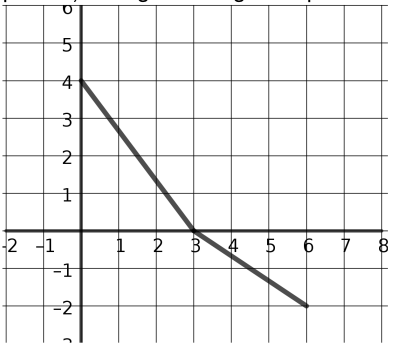
\includegraphics[scale=0.4]{2022juna.png}
\end{center}
a) Determine razonadamente el valor de la integral definida $\int_0^3 f(x)dx.$\\
b) ¿Cuál número es mayor,  $\int_0^3 f(x)dx$ o  $\int_0^6 f(x)dx$? Razone su respuesta.
\end{ejer}

\begin{ejer}\em (2021-2022)\\
Considere la función real de variable real dada por la siguiente expresión:
\[f(x)= \frac{x^3}{(x-K)^2}.\]
a) Obtenga el valor de la constante $K$ para que la recta tangente a la función en $x = 9$ sea paralela al eje de las $x.$ Indique la expresión de dicha recta.\\
b) Para $K = 3,$ señale los intervalos de crecimiento y decrecimiento de la función $f(x)$ y clasifique los extremos relativos de esta función.
\end{ejer}

\begin{ejer}\em (2021-2022)\\
La figura dada representa la gráfica de cierta función $f$
\begin{center}
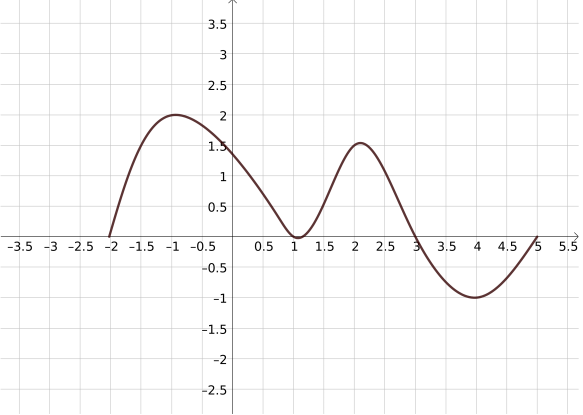
\includegraphics[scale=0.4]{2022jun.png}
\end{center}
La gráfica representada tiene tangentes horizontales en $x = -1, x = 1, x = 2$ y $x = 4.$\\
a) Determine razonadamente los intervalos en los que $f'(x) > 0.$\\
b) Determine razonadamente cuál es el signo de
\[\int_{-2}^5 f(x)dx.\]
\end{ejer}

\begin{ejer}\em (2021-2022)\\
Considere la función real de variable real
\[
f(x) = \frac{x^2-x+1}{x-1}
\]
a) Determine sus asíntotas (verticales, horizontales y oblicuas).\\
b) Calcule $f'(x)$ y halle el valor de $f'(2).$
\end{ejer}

\begin{ejer}\em (2021-2022)\\
Un escultor quiere dividir un alambre muy fino en dos trozos que se utilizarán para delimitar, respectivamente, un cuadrado y un rectángulo cuya base debe medir el doble que su altura. Posteriormente, se fabricarán ambas figuras planas con un material que cuesta 16 céntimos de euro$/cm^2$
para el cuadrado y 10 céntimos de euro$/cm^2$ para el rectángulo. Si el alambre inicial mide 450 cm, determine la función de coste total de ambas figuras. Obtenga la longitud de cada trozo de alambre para que el coste total de estas piezas sea mínimo.
Sugerencia: Exprese el coste total en función de la altura del rectángulo y utilice 3 cifras decimales para realizar los cálculos.
\end{ejer}


\begin{ejer}\em (2020-2021)\\
Dada la función real de variable real definida por:
\[
f(x)=\left \{ \begin{matrix}
x^2-x-1  & \text{si} & x\leq 3\\
\frac{3a}{x} & \text{si} & x> 3
\end{matrix}\right.
\]
a) Determine el valor del parámetro real $a$ para que la función $f(x)$ sea continua en todo su dominio. ¿Para ese valor de $a$ es $f(x)$ derivable?\\
b) Para $a=1,$ calcule la ecuación de la recta tangente a la gráfica de la función en el punto de abscisa $x=1.$
\end{ejer}

\begin{ejer}\em (2020-2021)\\
Se considera la función real de variable real $f(x)=\frac{x^3-2x^2}{(x-1)^2}$\\
a) Calcule el dominio y las asíntotas de $f(x).$\\
b) Determine sus intervalos de crecimiento y decrecimiento.
\end{ejer}

\begin{ejer}\em (2020-2021)\\
Se sabe que la derivada de una función real $f(x)$ de variable real es:
\[f'(x)=3x^2+8x\]
a) Determine la expresión de $f(x)$ sabiendo que $f(1)=11.$\\
b) Determine los máximos y mínimos locales de $f(x),$ si los hubiera.
\end{ejer}

\begin{ejer}\em (2020-2021)\\
Se considera la función real de variable real 
\[f(x)=\frac{x^3+4}{x^2-1}\]
a) Determine el dominio de $f(x)$ y calcule sus asíntotas.\\
b) Calcule la ecuación de la recta tangente a la gráfica de $f(x)$ en el punto de abscisa $x=0.$
\end{ejer}

\begin{ejer}\em (2020-2021)\\
Se considera la función real de variable real definida por:
\[
f(x)=\left \{ \begin{matrix}
x^2-ax & \text{si} & x\leq 1\\
ln(x) & \text{si} & x> 1
\end{matrix}\right.
\]
a) Determine para qué valores de $a\in\mathbb{R}$ la función $f(x)$ es continua en $\mathbb{R}.$\\
b) Para $a=1,$ halle el área de la región acotada delimitada por la función $f(x),$ el eje de abscisas y las rectas $x=-1, x=0.$ 
\end{ejer}

\begin{ejer}\em (2020-2021)\\
Se considera la función real de variable real, definida $f(x) = (x^2 - 3)e^x.$\\
a) Obtenga los intervalos de crecimiento y decrecimiento de $f(x)$ y determine sus extremos relativos indicando si corresponden a máximos o mínimos.\\
b) Calcule 
\[\int_1^2e^{-x}f(x)dx\]
\end{ejer}

\newpage

\begin{ejer}\em (2019-2020)\\
Se considera la función real de variable real
\[
f(x)=\left \{ \begin{matrix}
\frac{6x}{2x^2+1} & \text{si} & x< 1\\
2m+ln(x) & \text{si} & x> 1
\end{matrix}\right.
\]
a) Estudie los valores del parámetro $m\in\mathbb{R}$ para que $f (x)$ sea continua en $x = 1$ y calcule la derivada de la función para $x < 1 .$\\
b) Halle el área de la región del plano limitada por la curva $y = f (x) ,$ las rectas $x= -1$ y $x = 0$ y el eje 0X.
\end{ejer}

\begin{ejer}\em (2019-2020)\\
Se considera la función real de variable real definida por
\[f(x) =\frac{ax^2-3}{x^2-5}\]
a) Calcule el valor del parámetro $a\in \mathbb{R}$ para que $f (x)$ tenga una asíntota horizontal en $y = -1 .$\\
b) Para $a = 1,$ halle los intervalos de crecimiento y decrecimiento de $f (x)$ y los extremos relativos, si existen.
\end{ejer}

\begin{ejer}\em (2019-2020)\\
Dada la función real de variable real
\[f (x) = e^{2x} + x\]
a) Determine la ecuación de la recta tangente a $f (x)$ en $x = 0.$\\
b) Calcule
\[\int_0^1 f(x)dx\]
\end{ejer}

\begin{ejer}\em (2019-2020)\\
Se considera la función real de variable real definida por
\[f(x)=\frac{4x-x^3}{3x+x^2}+4\]
a) Calcule el dominio de la función y obtenga el valor que hay que asignar a $f (x)$ en $x = 0$ para que la función anterior sea continua en este punto.\\
b) Obtenga las asíntotas de esta función en caso de que existan.
\end{ejer}

\begin{ejer}\em (2019-2020)\\
Se considera la función real de variable real
\[f(x)=-x^4+x^3+2x^2\]
a) Determine la ecuación de la recta tangente a $f (x)$ en el punto de abscisa $x =-1.$\\
b) Obtenga el área del recinto acotado delimitado por la función $f(x)$ y el eje de abscisas para valores de $x > 0.$
\end{ejer}

\begin{ejer}\em (2019-2020)\\
Se considera la función real de variable real dada por la siguiente expresión:
\[f(x)=3(x+k)e^{\frac{-x}{2}}\]
a) Indique el dominio de la función y obtenga razonadamente el valor del parámetro real $k$ para que la tangente a la función en el punto de abscisa $x = 1$ sea horizontal. Determine también la ecuación de la recta tangente a
la función en dicho punto.\\
b) Para $k = 1,$ señale los intervalos de crecimiento y decrecimiento de $f (x).$
\end{ejer}

\newpage

\begin{ejer}\em (2018-2019)\\
Se considera la función real de variable real
\[
f(x)=\left \{ \begin{matrix}
\frac{x^3}{x^2-9} & \text{si} & x< 3,\\
x^2-4 & \text{si} & x\geq 3.
\end{matrix}\right.
\]
a) Estúdiese la continuidad de $f.$\\
b) Determínese si f tiene asíntotas horizontales, verticales u oblicuas.
\end{ejer}

\begin{ejer}\em (2018-2019)\\
Se considera la función real de variable real $f (x) = 2x^3 - 8x.$\\
a) Determínese en qué puntos la tangente a la curva $y = f(x)$ es horizontal.\\
b) Calcúlese el área de la región acotada del plano delimitada por la gráfica de $f,$ el eje de abscisas y las rectas $x = 0, x = 2.$
\end{ejer}

\begin{ejer}\em (2018-2019)\\
Se considera la función real de variable real definida por $f(x) = x^3 + x^2 - 5x + 3.$\\
a) Determínense los puntos de corte con los ejes de coordenadas así como los límites de la función cuando $x$ tiende a infinito y a menos infinito.\\
b) Determínense los valores de $x$ en los que la pendiente de la recta tangente a la función es igual a 3.
\end{ejer}

\begin{ejer}\em (2018-2019)\\
La derivada de una función real de variable real, f (x), viene dada por la expresión:
\[f'(x) = 2x^2 - 4x - 6\]
a) Obténgase la expresión de la función $f(x)$ sabiendo que pasa por el punto $(0, 3).$\\
b) Determínense los extremos relativos de la función $f(x)$ indicando si corresponden a máximos o mínimos relativos y estúdiese la concavidad $(\cup)$ y convexidad $(\cap)$ de esta función.
\end{ejer}

\begin{ejer}\em (2018-2019)\\
Se considera la función real de variable real:
\[f(x)=\frac{8}{x^2+4}\]
a) Determínense los intervalos de crecimiento y decrecimiento de $f(x)$ y obténganse sus asíntotas verticales y horizontales, si las tuviese.\\
b) Obténgase la ecuación de la recta tangente a la gráfica en el punto de abscisa $x = 2.$
\end{ejer}

\begin{ejer}\em (2018-2019)\\
La función real de variable real, $f(x),$ se define según la siguiente expresión:
\[
f(x)=\left \{ \begin{matrix}
e^x+k & \text{si} & x\leq 0,\\
1-x^2 & \text{si} & 0<x\leq 3,
\frac{1}{x-3} & \text{si} & x> 3.
\end{matrix}\right.
\]
a) Analícese la continuidad de la función en todo su dominio según los valores de $k.$\\
b) Considerando $k = 0,$ obténgase el área del recinto acotado delimitado por la función $f (x),$ el eje de abscisas y las rectas $x = - 1$ y $x = 1.$
\end{ejer}

\begin{ejer}\em (2017-2018)\\
Considérese la función real de variable real $f(x)=\frac{x}{1-4x^2}.$\\
a) Determínense los intervalos de crecimiento y decrecimiento de $f.$\\
b) Estúdiense las asíntotas de $f.$
\end{ejer}

\begin{ejer}\em (2017-2018)\\
Los beneficios, en millones de euros, de una determinada inversión vienen dados por la función $f(x) = x^3 - 12x,$ donde $x$ representa cierto índice que puede tomar cualquier valor real.\\
a) Determínese, en el caso de que exista, el valor del índice para el que el beneficio es mayor que el de todos los valores de un entorno suyo. ¿Cuál sería el beneficio para ese valor del índice?\\
b) Supóngase que el valor actual del índice es $x = 4$ y que está previsto que éste experimente un incremento positivo. Justifíquese si el beneficio aumentará o disminuirá.
\end{ejer}

\begin{ejer}\em (2017-2018)\\
Se considera la función real de variable real definida por:
\[
f(x)=\left \{ \begin{matrix}
x^3+2e^x & \text{si} & x< 0,\\
\frac{2}{3+x} & \text{si} & x\geq 0.
\end{matrix}\right.
\]
a) Determínense el dominio de $f (x)$ y estúdiese su continuidad.\\
b) Calcúlese $\int_{-1}^0f(x)dx.$
\end{ejer}

\begin{ejer}\em (2017-2018)\\
Dada la función real de variable real definida por:\[
f(x)=\left \{ \begin{matrix}
\frac{x+2}{x-1} & \text{si} & x\leq 2,\\
\frac{3x^2-2x}{x+2} & \text{si} & x>2.
\end{matrix}\right.
\]
a) Estúdiese si $f (x)$ es continua en $x = 2.$\\
b) Calcúlese la función derivada de $f (x)$ para $x < 2.$
\end{ejer}

\begin{ejer}\em (2017-2018)\\
Se considera la función real de variable real
\[f(x)=\frac{x^3}{(x+1)^2}\]
a) Calcúlense el dominio y las asíntotas de $f (x).$\\
b) Determínense sus intervalos de crecimiento y decrecimiento.
\end{ejer}

\begin{ejer}\em (2017-2018)\\
Se considera la función real de variable real:
\[f(x)=2x^3-5x^2+3x\]
a) Calcúlese el área del recinto acotado limitado por la gráfica de la función $f (x)$ y el eje OX.\\
b) Hállese la ecuación de la recta tangente a la gráfica de $f (x)$ en el punto de abscisa $x = 0.$
\end{ejer}

\begin{ejer}\em (2016-2017)\\
Se considera la función real de variable real:
\[
f(x)=\left \{ \begin{matrix}
ax+1 & \text{si} & x<-1,\\
x^2+x-2 & \text{si} & x\geq -1.
\end{matrix}\right.
\]
a) Calcúlese el valor del parámetro real $a$ para que $f (x)$ sea una función continua en todo su dominio.\\
b) Para $a = 2,$ calcúlense los puntos de corte de la gráfica de la función con los ejes cartesianos. Determínense sus intervalos de crecimiento y decrecimiento.
\end{ejer}

\begin{ejer}\em (2016-2017)\\
Se considera la función real de variable real
\[f(x)=\frac{x^2-1}{3x-2}\]
a) Estúdiense sus asíntotas.
b) Determínense los intervalos de crecimiento y decrecimiento de la función.
\end{ejer}

\begin{ejer}\em (2016-2017)\\
Se considera la función real de variable real
\[f(x)=x^2+ax\]
a) Calcúlese el valor del parámetro real $a$ para que la función $f (x)$ tenga un extremo relativo en $x = 2.$ Determínese si se trata de un máximo o un mínimo local.\\
b) Para $a = - 2,$ hállese el área del recinto acotado por la gráfica de $f(x),$ el eje de abscisas y las rectas $x = 0$ y $x = 2.$
\end{ejer}

\begin{ejer}\em (2016-2017)\\
a) Determínese el valor de la derivada de la función $f (x) =\frac{e^x}{1+x}$ en el punto de abscisa $x=0.$\\
b) Estúdiense las asíntotas de la función $f (x) =\frac{x^3}{1-x^2}.$
\end{ejer}

\begin{ejer}\em (2016-2017)\\
Considérese la función real de variable real:
\[f(x)=x^3-3x\]
a) Calcúlense $\lim_{x\to -\infty}\frac{f(x)}{1-x^3}$ y $\lim_{x\to 0} \frac{f(x)}{x}.$\\
b) Estúdiense los intervalos de crecimiento y decrecimiento de $f (x).$
\end{ejer}

\begin{ejer}\em (2016-2017)\\
Se considera la función real de variable real:
\[f(x)=\left \{ \begin{matrix}
\frac{2}{x+2} \text{ si } x\leq 0\\
x+2\text{ si } x>0
\end{matrix}\right.\]
a) Estúdiese la continuidad de $f (x)$ en $\mathbb{R}.$\\
b) Calcúlese $\int_{-1}^0f(x)dx.$
\end{ejer}

\begin{ejer}\em (2015-2016)\\
Dada la función real de variable real definida por
\[f(x)=\left \{ \begin{matrix}
x^2+1 & \text{ si } & x<1,\\
\frac{ax+b}{x} & \text{ si } & 1\leq x\leq 2,\\
\sqrt{x^3+1} & \text{ si } &x>2.
\end{matrix}\right.\]
a) Determínense los valores que deben tomar los parámetros $a$ y $b$ para que $f (x)$ sea continua en $x = 1$ y $x = 2.$\\
b) Calcúlese, para $a = 4$ y $b = - 2,$ el área del recinto acotado por la gráfica de $f(x),$ el eje de abscisas y las rectas $x = 1$ y $x = 2.$
\end{ejer}

\begin{ejer}\em (2015-2016)\\
Se considera la función real de variable real:
\[f(x)=\left \{ \begin{matrix}
x^2+2x & \text{ si } & x<0,\\
-x^2+3x & \text{ si } & x\geq 0.
\end{matrix}\right.\]
a) Estúdiese la continuidad y derivabilidad de la función.\\
b) Determínense los valores de $a\in\mathbb{R}$ para los cuales la pendiente de la recta tangente a la gráfica de $f (x)$ en el punto de abscisa $x = a$ es $m = -2.$ Calcúlese, para cada valor de a obtenido, la recta tangente a la gráfica de $f (x)$ en el punto de abscisa $x = a.$
\end{ejer}

\begin{ejer}\em (2015-2016)\\
Se considera la función real de variable real
\[f(x)=\frac{x^2-3}{x^2+9}.\]
a) Calcúlense sus asíntotas.\\
b) Determínense los intervalos de crecimiento y decrecimiento de la función.
\end{ejer}

\begin{ejer}\em (2015-2016)\\
Se considera la función real de variable real:
\[f(x)=x^3+8\]
a) Determínese el área de la región acotada delimitada por la gráfica de $f(x),$ el eje de abscisas y por las rectas $x = - 3$ y $x = - 1.$\\
b) Calcúlese la ecuación de la recta tangente a la gráfica de la función $f(x)$ en el punto de abscisa $x = 1.$
\end{ejer}

\begin{ejer}\em (2015-2016)\\
Se considera la función real de variable real
\[f(x)=\left \{ \begin{matrix}
\frac{-x+b}{x-2} & \text{ si } & x\leq -1,\\
\frac{x^2+6x+5}{x^2+4x+3} & \text{ si } & x>-1.
\end{matrix}\right.\]
a) Determínese para qué valores del parámetro $b$ la función $f(x)$ es continua en $x = -1.$\\
b) Calcúlense las asíntotas de $f(x).$
\end{ejer}

\begin{ejer}\em (2015-2016)\\
Sabiendo que la derivada de una función real de variable real es:
\[f'(x)=6x^2+4x-2.\]
a) Determínese la expresión de $f(x)$ sabiendo que $f (0) = 5.$\\
b) Determínense los intervalos de crecimiento y decrecimiento de la función $f$ así como sus máximos y mínimos locales, si los tuviese.
\end{ejer}

\begin{ejer}\em (2014-2015)\\
Se considera la función real de variable real definida por $f(x)=4x^3-ax^2-ax+2, a\in\mathbb{R}.$\\
a) Determínese el valor del parámetro real $a$ para que la función alcance un extremo relativo en $x = 1 / 2.$ Compruébese que se trata de un mínimo.\\
b) Para a = 2, calcúlese el valor de $\int_{-1}^1f(x)dx$
\end{ejer}

\begin{ejer}\em (2014-2015)\\
Se considera la función real de variable real
\[f(x)=-8x^2+24x-10\]
a) Calcúlense los máximos y mínimos locales de $f$ y represéntese gráficamente la función.\\
b) Determínese el área del recinto cerrado comprendido entre la gráfica de la función $f$ y las rectas $x = 1, x = 2$ e $y = 4.$
\end{ejer}

\begin{ejer}\em (2014-2015)\\
Considérese la función real de variable real
\[f(x)=\left \{ \begin{matrix}
e^x & \text{ si } & x<0,\\
\frac{x^3}{(x-2)^2} & \text{ si } & x\geq 0.
\end{matrix}\right.\]
a) Estúdiese la continuidad de esta función.\\
b) Determínense las asíntotas de esta función.
\end{ejer}

\begin{ejer}\em (2014-2015)\\
Sabiendo que la derivada de una función real de variable real $f$ es
\[f'(x)=3x^2+2x\]
a) Calcúlese la expresión de $f(x)$ sabiendo que su gráfica pasa por el punto $(1, 4).$\\
b) Calcúlese la ecuación de la recta tangente a la gráfica de la función $f$ en el punto $(1, 4).$
\end{ejer}

\begin{ejer}\em (2014-2015)\\
Sean las funciones reales de variable real
\[f(x)=x^2-6x \hspace*{5mm}\text{ y }\hspace*{5mm} g(x)=x-10\]
a) Represéntense gráficamente las funciones $f$ y $g.$\\
b) Calcúlese el área del recinto plano acotado por las gráficas de las funciones $f$ y $g.$
\end{ejer}

\begin{ejer}\em (2014-2015)\\
Se considera la función real de variable real definida por:
\[f(x)=\left \{ \begin{matrix}
\frac{x^2-4}{x^2-5x+6} & \text{ si } & x<2,\\
3x+m & \text{ si } & x\geq 2.
\end{matrix}\right.\]
a) Calcúlese el valor del parámetro real $m$ para que la función $f$ sea continua en $x = 2.$\\
b) Calcúlense $\lim_{x\to -\infty}f(x)$ y $\lim_{x\to +\infty}f(x)$
\end{ejer}

\begin{ejer}\em (2013-2014)\\
Se considera la función real de variable real definida por
\[f(x)=\frac{(x-3)^2}{x(x-2)}\]
a) Determínense las asíntotas de $f.$\\
b) Estúdiese si la función $f$ es creciente o decreciente en un entorno de $x=4.$
\end{ejer}

\begin{ejer}\em (2013-2014)\\
Se considera la función real de variable real definida por $f(x)=2e^{x+1}.$\\
a) Esbócese la gráfica de la función $f.$\\
b) Calcúlese el área del recinto acotado limitado por la gráfica de la función, el eje de abscisas y las rectas $x=0$ y $x=1.$
\end{ejer}

\begin{ejer}\em (2013-2014)\\
Se considera la función real de variable real definida por
\[f(x)=\frac{\lambda x}{4+x^2}\]
a) Calcúlese el valor del parámetro real $\lambda$ para que la reta tangente a la gráfica de $f$ en $x=-1$ sea paralela a la recta $y=2x-3.$\\
b) Calcúlese $\int_0^2f(x)dx$ para $\lambda=1.$
\end{ejer}

\begin{ejer}\em  (2013-2014)\\
Se considera la función real de variable real definida por $f(x)=\left \{ \begin{matrix}
x+a \text{ si } x<1\\
x^2-2\text{ si } 1\leq x\leq 3\\
x+b \text{ si } x>3.
\end{matrix}\right.
$\\
a) Determínense $a$ y $b$ para que $f$ sea continua en todo $\mathbb{R}.$\\
b) Calcúlese $\int_1^3 f(x)dx.$
\end{ejer}

\begin{ejer}\em (2013-2014)\\
Dada la función real de variable real $f(x)=4x^3-3x^2-2x.$
a) Determínese la ecuación de la recta tangente a la gráfica de $f$ en el punto de abscisa $x=1.$\\
b) Calcúlese $\int_2^3f(x)dx.$
\end{ejer}

\begin{ejer}\em (2013-2014)\\
Se considera la función real de variable real definida por 
\[f(x)=\frac{x^2}{x-2}\]
a) Determínense sus asíntotas.\\
b) Determínense el dominio y los intervalos de crecimiento y decrecimiento de $f.$
\end{ejer}


\begin{ejer}\em (2012-2013)\\
Se considera la función real de variable real definida por $f(x)=\frac{x^3}{x^2-9}$.\\
a) Hállense las asíntotas de $f$.\\
b) Determínese la ecuación de la recta tangente a la gráfica de  $f$ en el punto de abcisa $x=1$.
\end{ejer}

\begin{ejer}\em (2012-2013)\\
Se considera la función real de variable real definida por:
\begin{equation*}
f(x)=\left \{ \begin{matrix} ax^2-3 & \mbox{si } x\leq 1,
\\ \ln(2x-1) & \mbox{si } x > 1. \end{matrix}\right. 
\end{equation*}
a) Calcúlese $a$ para que la función $f$ sea continua en todo $\mathbb{R}$.\\
b) Represéntese gráficamente la función para el caso $a=3$.\\
Nota: $\ln x$ denota al logaritmo neperiano del número $x$.
\end{ejer}

\begin{ejer}\em (2012-2013)\\
Se considera la función real de variable real definida por $f(x)=\frac{x}{x^2+4}$.\\
a) Determínense los extremos relativos de $f$.\\
b) Calcúlese la integral definida $\int_0^1f(x)dx$.
\end{ejer}

\begin{ejer}\em (2012-2013)\\
Se considera la función real de variable real definida por $f(x)=3e^{-2x}$.\\
a) Obténgase la ecuación de la recta tangente al gráfica de $f$ en el punto $x=0$.\\
b) Calcúlese el área de la región plana acotada limitada por la gráfica de $f$, las rectas $x=0,x=0,5$ y el eje de abcisas.
\end{ejer}

\begin{ejer}\em (2012-2013)\\
Se considera la función real de variable real
\begin{equation*}
f(x)=\left \{ \begin{matrix} e^x & \mbox{si } x<0,
\\ \frac{a+3x}{x^2-4x+3} & \mbox{si } x \geq 0. \end{matrix}\right. 
\end{equation*}
a) Estúdiese la continuidad de $f$ en $x=0$ para los distintos valores de $a$.\\
b) Determínense las asíntotas de la función.
\end{ejer}

\begin{ejer}\em (2012-2013)\\
Se considera la función real de variable real definida por $f(x)=x(5-x)^2$.\\
a)Determínense los intervalos de crecimiento y decrecimiento de $f$.\\
b)Determínense los intervalos de concavidad y convexidad de $f$.
\end{ejer}

\begin{ejer}\em (2011-2012) [3 puntos]\\
Se considera la función real de variable real definida por:$f(x)=\frac{x(2x-1)}{x-1}.$
a) Determínense las asíntotas de $f$. Calcúlense los extremos relativos de $f$.\\
b) Represéntese gráficamente la función $f$.\\
c) Calcúlese $\int_2^5\frac{f(x)}{x^2}dx$.
\end{ejer}

\begin{ejer}\em (2011-2012)[3 puntos]\\
Se considera la función real de variable real definida por:
\begin{equation*}
f(x)=\left \{ \begin{matrix} ax+b & \mbox{si } x\leq 1,
\\ x^3-x^2+1 & \mbox{si } x > 1. \end{matrix}\right. 
\end{equation*}
a) Calcúlense los valores de $a,b$ para los que la función $f$ es continua y derivable.\\
b) Para $a=0$ y $b=1,$ hállese la ecuación de la recta tangente a la gráfica de $f$ en los puntos en los que dicha tangente es paralela a la recta $y-8x=1$.\\
c) Sea $g$ la función real de variable real definida por $g(x)=1-2x^2$. Para $a=1$ y $b=0$, calcúlese el área de la región plana acotada limitada por la gráfica de $f$ y la gráfica de  $g$.
\end{ejer}

\begin{ejer}\em (2011-2012) [3 puntos]\\
Una empresa vinícola tiene plantadas 1200 cepas de vid en una finca, produciendo cada cepa una media de $16kg$ de uva. Existe un estudio previo que garantiza que por cada cepa que se añade a la finca, las cepas producen de media $0,01kg$ menos de uva cada una. Determínese el número de cepas que se deben añadir a las existentes para que la producción de uvas de la finca sea máxima.
\end{ejer}


\begin{ejer}\em (2011-2012) [3 puntos]\\
Se considera la función real de variable real definida por:
\begin{equation*}
f(x)=\left \{ \begin{matrix} x^2-4x+3 & \mbox{si } x\leq 1,
\\ -x^2+4x-3 & \mbox{si } x > 1. \end{matrix}\right. 
\end{equation*}
a) Estúdiese la continuidad y derivabilidad de la función $f$.\\
b) Represéntese gráficamente la función $f$.\\
c) Calcúlese el área del recinto plano acotado limitado por la gráfica de $f$, el eje OX, el eje OY y la recta $x=2$.
\end{ejer}

%%

\begin{ejer}\em (2010-2011)\\%
Se considera la función real de variable real definida por:
$$
f(x)=\frac{3x}{x^2-2}.
$$
a) Especifíquese su dominio de definición y los puntos de corte de la gráfica $f$ con los ejes coordenados. Determínense las asíntotas de $f$.\\
b) Determínese la ecuación de la recta tangente a la gráfica de $f$ en el punto de abcisa $x=1$.\\
c) Calcúlese la integral definida $\int_2^3f(x)dx$.
\end{ejer}

\begin{ejer}\em (2010-2011)\\%
Se considera la función real de variable real definida por:
\begin{equation*}
f(x)=\left \{ \begin{matrix} \frac{a}{x} & \mbox{si } x\leq -1,
\\ \frac{x^2-b}{4} & \mbox{si } x > -1. \end{matrix}\right. 
\end{equation*}
a) Calcúlense los valores de $a,b$ para que la función $f$ sea continua y derivable en $x=-1$.\\
b) Para $a=1,b=3,$ represéntese gráficamente la función $f$.\\
c) Calcúlese el valor de $b$ para que $\int_0^3f(x)dx=6$.
\end{ejer}

\begin{ejer}\em (2010-2011)\\
Se considera la función real de variable real definida por: $f(x)=\frac{(x+1)^2}{x^2+1}.$\\
a) Determínense las asíntotas de $f.$ Calcúlense los extremos relativos de $f.$\\
b) Represéntese gráficamente la función $f.$\\
c) Calcúlese el área del recinto plano acotado limitado por la gráfica de $f,$ la recta horizontal $y=1,$ la recta vertical $x=1.$
\end{ejer}

\begin{ejer}\em (2010-2011)\\
Se considera un rectángulo $R$ de lados $x,y.$\\
a) Si el perímetro de $R$ es igual a 12 m, calcúlense $x,y$ para que el área de $R$ sea máxima y calcúlese el valor de dicha área máxima.\\
b) Si el área de $R$ es igual a $36 m^2,$ calcúlense $x,y$ para que el perímetro de $R$ sea mínimo y calcúlese el valor de dicho perímetro mínimo.
\end{ejer}


\begin{ejer}\em (2009-2010)\\
Se considera la función real de variable real definida por:
\begin{equation*}
f(x)=\left \{ \begin{matrix} x+4 & \mbox{si } x<0,
\\ 4-x^2 & \mbox{si } 0\leq x\leq 2,
\\ ax+b & \mbox{si } x>2. \end{matrix}\right. 
\end{equation*}
a) Calcúlense $a,b$ para que la función $f$ sea continua y derivable en $x=2$.\\
b) Determínese la ecuación de la recta tangente a la gráfica de la función $f$ en el punto $x=1$.\\
c) Para $a=1,b=-2$, calcúlese el área de la región acotada limitada por la gráfica de $f$ y el eje OX.
\end{ejer}

\begin{ejer}\em (2009-2010)\\%
Se considera la función real de variable real definida por:
\begin{equation*}
f(x)=\left \{ \begin{matrix} -x^2-x+a & \mbox{si } x\leq 1,
\\ \frac{3}{bx} & \mbox{si } x>1. \end{matrix}\right. 
\end{equation*}
a) Calcúlense los valores de $a,b$ para que la función $f$ sea continua y derivable en todos los puntos.\\
b) Para $a=6,b=3/4,$ determínense los puntos de corte de la gráfica de $f$ con el eje OX.\\
c) Para $a=6,b=3/4,$ calcúlese el área del recinto plano acotado limitado por la gráfica de $f$, el eje OX y la recta vertical $x=2$.
\end{ejer}

\begin{ejer}\em (2009-2010)\\%
Se considera la función real de variable real definida por:
\begin{equation*}
f(x)=\left \{ \begin{matrix} x^2+1 & \mbox{si } x<0,
\\ ax+b & \mbox{si } 0\leq x\leq 3,
\\ x-5 & \mbox{si } x>3. \end{matrix}\right. 
\end{equation*}
a) Calcúlense los valores de $a,b$ para que la función $f$ sea continua en todos los puntos.\\
b) ¿Existen valores de  $a,b$ para los cuales $f$ es derivable en $x=3$? Razónese la respuesta.\\
c) Para $a=4,b=-1,$ calcúlese la integral definida $\int_{-1}^2f(x)dx$.
\end{ejer}

\begin{ejer}\em (2009-2010)\\
Se considera el rectángulo $(R)$ con vértices $BOAC$ con $B(0,b)$, $O(0,0)$, $A(a,0)$, $C(a,b)$, $a>0,b>0$, y cuyo vértice $C$ está situado en la parábola de ecuación $y=-x^2+12$.\\
a) Para $a=3$, determínense las coordenadas de los vértices de $(R)$ y calcúlese el área de $(R)$.\\
b) Determínense las coordenadas de los vértices de $(R)$ de manera que el área de $(R)$ sea máxima.\\
c) Calcúlese el valor de dicha área máxima.
\end{ejer}

\begin{ejer}\em (2009-2010)\\
El coste de un marco para una ventana rectangular es de 50 euros por cada metro de lado vertical y de 25 euros por cada metro de lado horizontal. Se desea construir una ventana de superficie igual a $2m^2$. Calcúlense sus dimensiones (largo y alto) para que el marco sea lo más barato posible. Calcúlese el precio mínimo del marco de dicha ventana.
\end{ejer}

\begin{ejer}\em (2009-2010)\\%
Se considera la función real de variable real definida por: 
$$
f(x)=\frac{x^2}{x-1}.
$$
a) Determínense sus asíntotas.\\
b) Calcúlense sus máximos y mínimos locales. Esbócese la gráfica de $f$.\\
c) Calcúlese el área del recinto plano acotado limitado por las rectas verticales $x=2,x=3$, la gráfica de la función $f$ y la recta de ecuación $y=x+1.$
\end{ejer}

\begin{ejer}\em (2009-2010)\\%
Se considera la función real de variable real definida por:
\begin{equation*}
f(x)=\left \{ \begin{matrix} 2x^2-a & \mbox{si } x\leq -1,
\\ -3x^2+b & \mbox{si } -1<x<1,
\\ \log x+a & \mbox{si } x\geq 1. \end{matrix}\right. 
\end{equation*}
a) Calcúlense los valores de $a,b$ para que la función $f$ sea continua en todos los puntos.\\
b) Para $a=0,b=3,$ represéntese gráficamente la función $f$.\\
c) Para $a=0,b=3,$ calcúlese la integral definida $\int_{-1}^1f(x)dx$.
\end{ejer}

\begin{ejer}\em (2009-2010)\\%
Se considera la función real de variable real definida por:
$$
f(x)=x^3-3x^2+4.
$$
a) Determínese la ecuación de la recta tangente a la gráfica de $f$ en su punto de inflexión.\\
b) Determínense los extremos relativos de $f$ y esbócese su gráfica.\\
c) Calcúlese el área del recinto plano acotado limitado por la gráfica de $f$ y la recta de ecuación $y=x+1$.
\end{ejer}

\begin{ejer}\em (2008-2009)\\%
El beneficio semanal (en miles de euros) que obtiene una central lechera por la producción de leche desnatada está determinado por la función
$$
B(x)=-x^2+7x-10
$$
en la que $x$ representa los hectolitros de leche desnatada producidos en una semana.\\
a) Represéntese gráficamente la función $B(x)$ con $x\geq 0$.\\
b) Calcúlense los hectolitros de leche desnatada que debe producir cada semana la central lechera para maximizar su beneficio. Calcúlese dicho beneficio máximo.\\
c) Calcúlese las cantidades mínima y máxima de hectolitros de leche desnatada que debe producir la central lechera cada semana para no incurrir en pérdidas (es decir, beneficio negativo).
\end{ejer}

\begin{ejer}\em (2008-2009)\\%
Se considera la función real de variable real definida por:
$$
f(x)=(x^2-1)^2.
$$
a) Determínense los extremos relativos de $f$.\\
b) Hállese la ecuación de la recta tangente a la gráfica de $f$ en el punto de abcisa $x=3$.\\
c) Calcúlese el área del recinto plano acotado limitado por la gráfica de  $f$ y el eje OX.
\end{ejer}

\begin{ejer}\em (2008-2009)\\
Se considera la función real de variable real definida por:
$$
f(x)=\frac{2x-1}{x^2-x-a}.
$$
a) Determínense las asíntotas de $f$, especificando los valores del parámetro real $a$ para los cuales $f$ tiene una asíntota vertical, dos asíntotas verticales o bien no tiene asíntotas verticales.\\
b) Para $a=-1$, calcúlense los valores de $b$ para los cuales se verifica que $\int_0^b f(x)dx=0$.
\end{ejer}

\begin{ejer}\em (2008-2009)\\%
Se considera la función real de variable real definida por:
\begin{equation*}
f(x)=\left \{ \begin{matrix} 2x+24 & \mbox{si } x\leq -3,
\\ x^2+9 & \mbox{si } -3<x\leq 2
\\ -x+15 & \mbox{si } x>2. \end{matrix}\right. 
\end{equation*}
a) Represéntese gráficamente la función $f$.\\
b) Hállese la ecuación de la recta tangente a la gráfica de $f$ en el punto de abcisa $x=1$.\\
c) Calcúlese el área del recinto plano acotado limitado por la gráfica de $f$ y el eje OX.
\end{ejer}

\begin{ejer}\em  (2007-2008)\\
Se desea fabricar un acuario con base cuadrada y sin tapa, de capacidad $500 dm^3$. La base y las paredes del acuario han de estar realizadas en crista. ¿Cuáles deben ser sus medidas para minimizar la superficie total del cristal empleado?
\end{ejer}

\begin{ejer}\em (2007-2008)\\%
Se considera la función real de variable real definida por:
$$
f(x)=\frac{x^2+x+2}{x}, \quad x\neq 0.
$$
a) Determínese las asíntotas de $f$.\\
b) Calcúlense su máximos y mínimos relativos y determínense sus intervalos de crecimiento.\\
c) Calcúlese la integral definida $\int_1^2 f(x)dx$.
\end{ejer}

\begin{ejer}\em (2007-2008)\\%
Se considera la función real de variable real definida por:
$$
f(x)=\frac{x^2+2}{x^2-4}, \quad x\neq \pm 2.
$$
a) Determínense las asíntotas de $f$.\\
b) Calcúlense los máximos y mínimos relativos de $f$ y determínense sus intervalos de crecimiento.\\
c) Calcúlese la integral definida:$\int_3^5(x^2-4)f(x)dx$.
\end{ejer}


\begin{ejer}\em (2007-2008)\\
Calcúlese el área de la región plana acotada limitada por las gráficas de las funciones reales de variable real:
$$
f(x)=x^2-x, \quad g(x)=1-x^2.
$$
\end{ejer}

\begin{ejer}\em (2006-2007)\\
Dada la función real de variable real definida por
$$
f(x)=\frac{(x-3)^2}{x+3}
$$
a) Determinar las asíntotas de la función.\\
b) Calcular sus máximos y sus mínimos y determinar sus intervalos de crecimiento.
\end{ejer}

\begin{ejer}\em (2006-2007)\\
Representar gráficamente la región acotada limitada por las gráficas de las funciones
$$
f(x)=\frac{5}{4}x^2 \quad g(x)=\frac{1}{2}(5x+20) \quad h(x)=\frac{1}{2}(-5x+20)
$$
y obtener su área.
\end{ejer}

\begin{ejer}\em (2006-2007)\\
La gráfica de la función $f(x)=ax^3+bx^2+c$ satisface las siguientes propiedades:
\begin{itemize}
\item[$\circ$] Pasa por el punto $(0,0)$.
\item[$\circ$] Tiene un máximo local en el punto $(1,2)$.
\end{itemize}
Se pide:\\
a) Obtener el valor de los coeficientes $a$,$b$ y $c$.\\
b) Hallar el área acotada del plano limitada por la gráfica de la función $g(x)=-x^3+3x$, el eje OX y la recta $x=1$.
\end{ejer}

\begin{ejer}\em (2006-2007)\\
Dada la función real de variable real definida por
$$
f(x)=\frac{x^2-x}{x^2-3x+2}
$$
a) Especificar su dominio de definición.\\
b) Estudiar su continuidad.\\
c) Calcular sus asíntotas, si las hubiera.
\end{ejer}


\begin{ejer}\em (2020-2021)%Modelo
Se considera la función real de variable real definida por
\[
f(x)=\left \{ \begin{matrix}
x^2+ax-\frac{1}{9}  & \text{si} & x\leq 0\\
\frac{x+1}{x^2-9} & \text{si} & x> 0
\end{matrix}\right.\]

a) Determine el dominio de $f(x)$ y calcule el valor del parámetro $a\in \mathbb{R}$ para que $f(x)$ sea derivable en todo su dominio.\\
b) Para $a = 0$ determine, si existen, las asíntotas de $f(x).$
\end{ejer}


\begin{ejer}\em (2020-2021)\\%Modelo
Dada la función
\[f (x) = x +\frac{4}{x^2}\]

a) Halle el dominio de la función y sus asíntotas.\\
b) Determine los intervalos de crecimiento y decrecimiento de la función y, si los hubiera, sus extremos relativos.
\end{ejer}

\begin{ejer}\em (2020-2021)\\%juna
Sea $f (x) = x^2 + ax$ donde a es un parámetro real.\\
a) Determine el valor de a para que la función $f (x)$ tenga una primitiva $F (x)$ que verifique $F (0) = 3$ y $F (2) = 9.$\\
b) Para $a = - 2,$ calcule el área de la región acotada del plano delimitada por la gráfica de $f (x),$ el eje de abscisas y las rectas $x = 0, x = 3.$
\end{ejer}



\end{document}

\begin{ejer}\em ()\\

\end{ejer}
